
Lorsque l'on veut adapter un système existant qui fonctionne sur une machine pour le faire fonctionner sur une autre machine, on dit qu'on \textbf{porte} un système. C'est ce qui a été envisagé dans ce projet.\\
\textit{Milkymist} est un système dont le code HDL et le code \languagetoto{C} du système d'exploitation sont totalement OpenSource et donc réutilisables et modifiables.\\
L'INSA dispose de cartes de développement \nexys. Cette carte ressemble à une \textit{Milkymist One} car elles sont toutes les deux dotées d'une puce \fpga{} Spartan6 et ont des périphériques communs tels que la mémoire et l'UART.\\

Le projet consiste donc au portage de l'architecture (figure \ref{milky-archi}) et du système logiciel \textit{Milkymist} en laissant de côté le multimédia pour avoir un système embarqué fonctionnel sur la \nexys qui permettrait par la suite de tester la technologie récente appelée \english{partial reconfiguration} par \brand{Xilinx} et dont l'abréviation est \textbf{PR}.

\begin{figure}[h!]
\centering
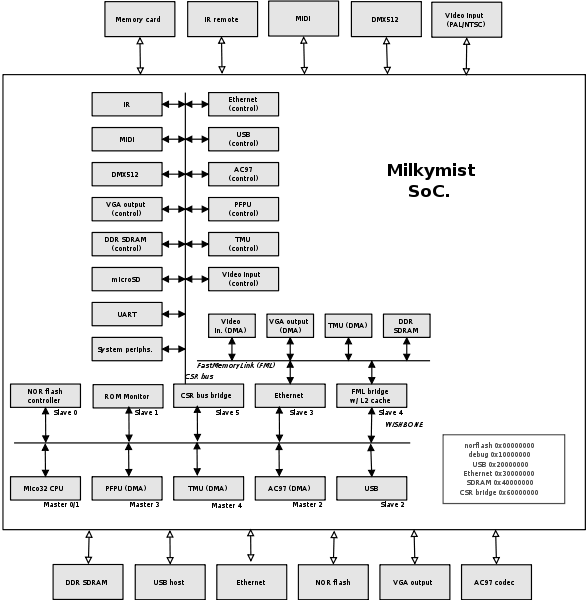
\includegraphics[scale=0.7]{milky_archi.png}
\caption{Architecture du système Milkymist}
\label{milky-archi}
\end{figure}

\subsection{La simulation sous Qemu}

Le but de cette partie était d'adapter le noyau linux (uClinux) de \textit{Milkymist} en se basant sur le portage réalisé par \brand{Theobroma-Systems}. Il nous fallait aussi créer un système de fichier minimal associé à ce noyau. Nous avons rencontré de problèmes liés aux outils de compilations. Ces bugs liés aux outils de compilations ont été corrigés. Une fois ce correctif appliqué, nous avons créé le système de fichier à l'aide d'\textit{OpenWrt}, qui a pour but de simplifier l'utilisation de linux sur différentes platforme, dont la carte de \textit{Milkymist}.\\
La création d'un noyau et d'un système de fichiers a donc été un succès et cela malgré le temps passé à bloquer à cause d'erreurs dans les outils de compilation.

\subsection{Le système sur cible réelle}

Dans un second temps, il nous fallait démarrer le noyau sur la \nexys{}. Nous avons dû modifier le code source du BIOS fourni par \textit{Milkymist} pour pouvoir démarrer le noyau présent en mémoire Flash. Le noyau est chargé via un outil JTAG développé par nos soins. Le BIOS doit ensuite le démarrer.\\

Nous avons rencontrés des problèmes lors du débogage du noyau à cause d'erreurs rendant l'affichage inopérant cela nous empêchant de détecter précisément leurs causes. De même, la modification du BIOS a été d'autant plus complexe que nous ne l'avions pas écrit. En effet, nous nous contentions de commenter ou de décommenter du code. Cependant, nous avons pu vérifier le bon fonctionnement des procédures de démarrage du noyau et en déduire que les erreurs se situaient à sa compilation. 



\section{Tests du matériel}

\subsection{La PSRAM}

Suite à des problèmes d'exécution du bios puis de démarrage de uClinux, nous avons tout d'abord voulu regarder si le contenu de la RAM était correct. Pour cela, nous souhaitions faire une simulation globale du système et regarder le contenu de la RAM. Or sur la \nexys{}, la RAM est un périphérique externe et n'a donc pas de relation avec le code HDL, elle est seulement connecté au reste par un contrôleur en Verilog. La première étape a consisté au remplacement de ce module par un module appelé BRAM codé en Verilog (RAM réalisé en portes logiques dans le FPGA) qui allait pouvoir être simulé.\\
Une fois cette tâche réalisée, nous avons voulu vérifier qu'il ne s'agissait pas d'un problème de communication avec le bus et que les signaux étaient corrects. Le problème pouvait également venir du module multiplexeur qui permet de sélectionner la mémoire soit flash soit RAM car leur bus de données est partagé.

\subsection{Simulation du système complet}

Cette simulation ne s'est pas révélée si aisée qu'on le pensait. Le système a une taille considérable et simuler seulement 0.2s nécessitait plusieurs minutes et une cinquantaine de gigaoctets. Finalement, après de multiples problèmes de compilation après modifications du testbench original, nous avons préféré abandonner. Comme le montre le schéma à la figure \ref{milky-archi}, l'architecture comprend trois bus différents, ce qui n'était pas du tout justifié pour notre projet et compliquait énormément notre tâche. Le bus Wishbone aurait seul suffit.